\documentclass[../rapport_MVEX01-11-05]{subfiles}
\begin{document}

\section{$k$-nearest-neighbours}\label{sec:knn}

\knn eller $k$-närmsta-grannar är en konceptuellt enkel modellfri
klassificeringsmetod.
Den baseras på prototypobjekt i egenskapsrummet och tilldelar en klass
till en observerad punkt baserat på dess närmsta grannar i egenskapsrummet.

Avståndet som används är vanligtvis det euklidiska, dvs
\begin{equation*}
    d(i) = \left(\sum_{i=1}^n(x_i-x_0,i)^2\right)^{1/2}
\end{equation*}
där $n$ är dimensionen på egenskapsrummet, $\vect{x}$ är koordinaterna för en
prototyp och $\vect{x_0}$ är observationen. Genom en sökning i
egenskapsrummet letar vi efter de $k$ närmsta grannarna. Om $k$ är större än ett
avgörs klasstillhörigheten genom majoritetsomröstning, dvs. den klass med flest
nära grannar vinner, se figur \ref{fig:knn-overview}.

\begin{figure}[!htb]
    \begin{center}
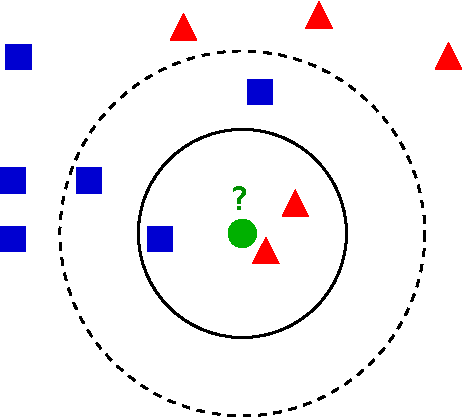
\includegraphics[width=0.5\textwidth]{bilder/KnnClassification}
    \end{center}
    \caption{kNN-klassificering av den runda observationen i mitten i ett rum
    med två klasser, trianglar och kvadrater. Majoritetsomröstning
    med $k=3$ leder till att den runda klassas som triangel, medan $k=5$ leder
    till klassificering som kvadrat.}
    \label{fig:knn-overview}
\end{figure}

Prototypobjekten är redan klassificerade objekt som väljs ur en inlärningsmängd.
De kan skrivas som
\begin{equation*}
    (\vect{x}_i, l_i)\qquad l_i \in \{ 1,\dotsc,K \}
\end{equation*}
där $l_i$ är en klassetikett och $K$ är antalet klasser.
Prototyperna kan väljas genom mer eller mindre sofistikerade metoder.
Exempelvis kan varje redan klassificerad punkt undersökas med \knn mot
alla andra punkter, varpå den tas bort ur mängden om den nya klassen avviker
från den ursprungliga.

Klasserna motsvarar sammanhanget olika statiska gester,
eller olika grupperingar i egenskapsrummet. För
varje observerad bildruta undersöker man alltså vilken klass den tillhör.

För att metoden ska fungera krävs att alla klasser är representerade med lika
många prototypobjekt, annars får vissa klasser större vikt och kommer med högre
sannolikhet att väljas. (Klasserna kan fortfarande viktas i efterhand.)
Om prototyperna är väl valda avspeglar de den sanna
förderlningen hos klassen.
Den är därför ofta att föredra framför en Gaussian Mixture Model, där
varje klass approximeras av sina anpassade parametrar.
\cite{Hastie09}.

\subsection{Algoritmer för \knn}
Att linjärt söka genom prototypmängden tar enligt
\citeasnoun{Roding08} lång tid ($\mathcal{O}(d k n)$).
Istället kan man, beroende på mängdens storlek och antalet egenskaper,
använda smartare metoder.
Ett tillvägagångssätt är att inte söka de sanna närmsta grannarna,
utan att med en slumpmässig metod approximera till önskad noggranhet.
Detta tillåter stora datamängder och hög dimension.

En metod som är snabb för dimensioner lägre än ungefär 20 är kd-tree.
Den går ut på att prototypmängden delas av plan genom egenskapsrummet,
som resulterar i ett binärt träd. Färdiga implementeringar finns dessutom
i överflöd \cite{Skiena08}.

%Detta måste givetvis göras en gång per gest, vilket ger oss en kodbok
%per gest; detta eftersom vi har en HMM per gest.
%
%\marginpar{Eller, hur ska vi göra egentligen? En eller flera
% kodböcker? Hur skalar algoritmerna, hur jobbigt blir det? Säger
% någon referens något om detta?}

%FIGUR
%http://en.wikipedia.org/wiki/File:KnnClassification.svg

\end{document}
